\documentclass[12pt,a4paper]{article}

% ===== PAKETE =====
\usepackage[ngerman]{babel}          % Deutsche Sprache
\usepackage[utf8]{inputenc}          % UTF-8 Kodierung
\usepackage[T1]{fontenc}             % Schriftkodierung
\usepackage{lmodern}                 % Schönere Schrift
\usepackage[left=2.5cm,right=2.5cm,top=2.5cm,bottom=2.5cm]{geometry}

% Layout & Formatierung
\usepackage{setspace}                % Zeilenabstand


\usepackage{parskip}                 % Absatzformatierung
\usepackage{fancyhdr}                % Kopf- und Fußzeilen

% Bilder & Grafiken
\usepackage{graphicx}                % Bilder einbinden
\usepackage{float}                   % Bessere Positionierung
\usepackage{caption}                 % Bildunterschriften

% Tabellen
\usepackage{tabularx}                % Flexible Tabellen
\usepackage{booktabs}                % Schönere Tabellen

% PDF einbinden
\usepackage{pdfpages}                % Für Deckblatt

% Mathematik (falls benötigt)
\usepackage{amsmath}
\usepackage{amssymb}
\usepackage{siunitx}

% Links & Verweise
\usepackage{hyperref}                % Klickbare Links
\hypersetup{
    colorlinks=true,
    linkcolor=black,
    citecolor=black,
    urlcolor=blue,
    pdftitle={Titel deiner Arbeit},
    pdfauthor={Dein Name}
}

% Literaturverzeichnis
\usepackage[backend=biber,style=numeric,sorting=nty]{biblatex}
\addbibresource{literatur.bib}

% ===== EINSTELLUNGEN =====
\onehalfspacing                      % 1,5-facher Zeilenabstand
\setlength{\parindent}{0pt}          % Keine Einrückung
\pagenumbering{arabic}

% Kopf- und Fußzeilen
\pagestyle{fancy}
\fancyhf{}
\fancyhead[L]{\leftmark}
\fancyhead[R]{\thepage}
\renewcommand{\headrulewidth}{0.4pt}

% ===== DOKUMENT =====
\begin{document}

% Vorgegebenes Deckblatt einbinden
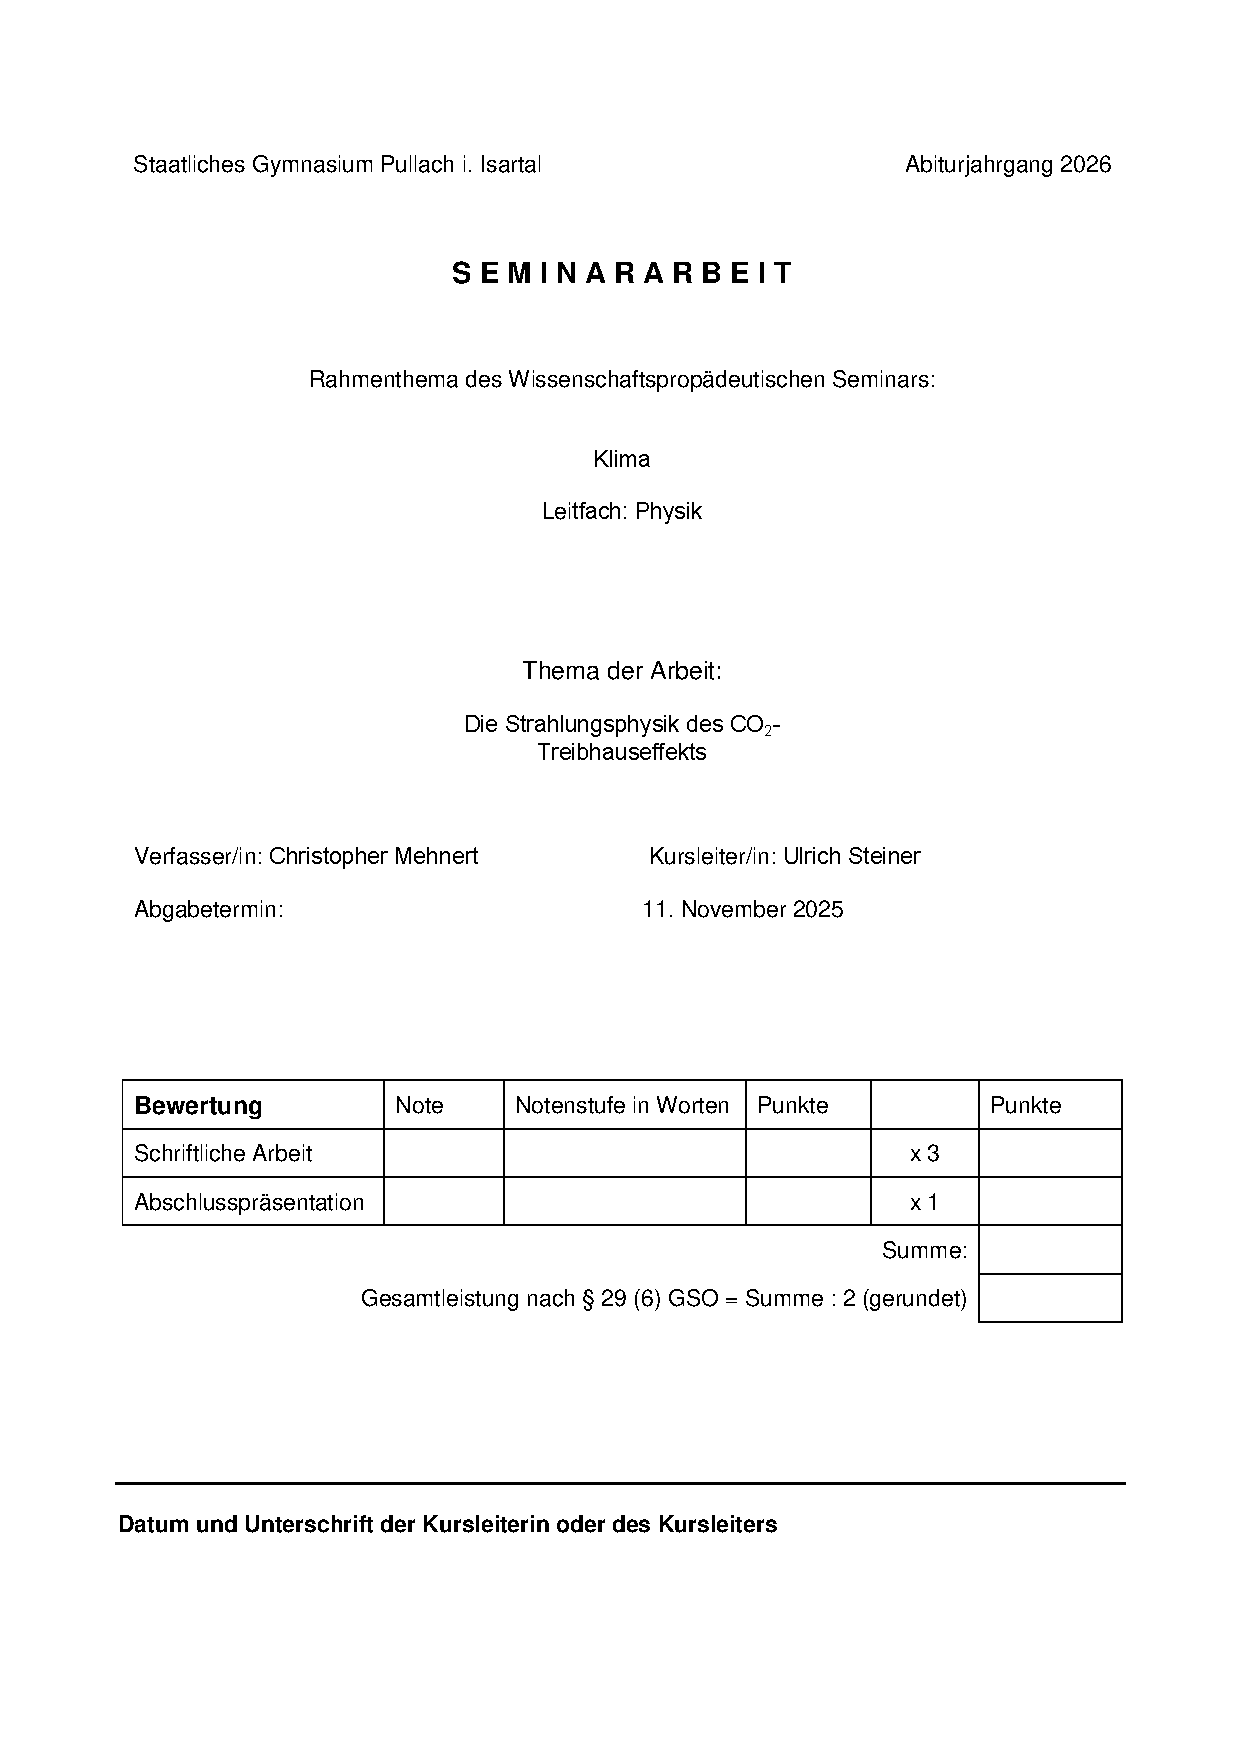
\includepdf[pages={1,2,3}]{assets/deckblatt.pdf}


% Inhaltsverzeichnis
\setcounter{page}{2}
\tableofcontents
\newpage

% Optional: Abbildungsverzeichnis
% \listoffigures
% \newpage

% Optional: Tabellenverzeichnis
% \listoftables
% \newpage

% ===== HAUPTTEIL =====

\section{Einleitung}

\section{Physikalische Grundlagen der Wärmestrahlung}

\subsection{Strahlungsgesetze}
Jedes Medium emittiert elektromagnetische Strahlung zufällig in alle Richtungen. 
Die Intensität dieser Emission hängt sowohl von der Temperatur als auch von den Materialeigenschaften des Mediums ab. 
Der von einer Oberfläche abgegebene Strahlungswärmestrom wird als \textit{spezifische Ausstrahlung} bezeichnet.

Dabei wird zwischen der \textit{gesamten spezifischen Ausstrahlung} $E$ und der \textit{spektralen spezifischen Ausstrahlung} $E_f$ unterschieden:
\begin{align*}
E_f &\equiv \text{abgestrahlte Energie pro Zeit, Oberfläche und Frequenz.} \\
E &\equiv \text{abgestrahlte Energie pro Zeit und Oberfläche.}
\end{align*}
\cite[S.~6--7]{radiativeHeatTransfer}


\subsubsection{Das Plancksche Strahlungsgesetz}

Die spektrale spezifische Ausstrahlung eines ideal schwarzen Körpers $E_b$ wird durch das Plancksche Strahlungsgesetz beschrieben. 
Es gibt an, wie viel Energie pro Zeit, Fläche und Frequenzintervall von einer ideal schwarzen Oberfläche bei einer bestimmten Temperatur $T$ emittiert wird. 
Dieses Gesetz wurde 1900 von Max Planck \cite{plancknormalspektrum} hergeleitet und ist heute als \textit{Plancksches Strahlungsgesetz} bekannt. 
Für eine schwarze Oberfläche, die an ein transparentes Medium mit dem Brechungsindex $n$ grenzt, ergibt sich die spektrale spezifische Ausstrahlung\cite[S.7]{radiativeHeatTransfer} zu:

\begin{equation}
  \label{Plancksche Ausstrahlung Frequenz mit Brechungsindex}
  E_{bf}(T, f) = \frac{2\pi h f^3 n^2}{c_0^2} \cdot \frac{1}{e^{hf/kT}-1} 
  \quad \text{\cite[S.8]{radiativeHeatTransfer}}
\end{equation}

Zur Vereinfachung wird angenommen, dass der Brechungsindex $n = 1$ beträgt, da sich die betrachteten Vorgänge im Vakuum oder in Luft abspielen, wo dieser Wert nahezu identisch ist.

\begin{equation}
  \label{Plancksche Ausstrahlung Frequenz}
  E_{bf}(T, f) = \frac{2\pi h f^3}{c_0^2} \cdot \frac{1}{e^{hf/kT}-1} 
\end{equation}


Das Plancksche Strahlungsgesetz lässt sich auch in Abhängigkeit von der Wellenlänge $\lambda$ formulieren:

\begin{equation}
  \label{Plancksche Ausstrahlung Wellenlänge}
  E_{b\lambda}(T, \lambda) = \frac{2\pi h c_0^2}{\lambda^5} \cdot \frac{1}{e^{hc_0/\lambda kT}-1}
\end{equation}

Dabei bezeichnet $h = \SI{6.626e-34}{\joule\second}$ das Plancksche Wirkungsquantum, 
$c_0 = \SI{2.998e8}{\meter\per\second}$ die Lichtgeschwindigkeit im Vakuum 
und $k = \SI{1.381e-23}{\joule\per\kelvin}$ die Boltzmann-Konstante \cite{codata2018}.

\subsubsection{Das Stefan-Boltzmann Gesetz}
Die Integration der spektralen spezifischen Ausstrahlung über das gesamte 
elektromagnetische Spektrum liefert die \textit{Gesamtausstrahlung} $E$:
\begin{equation}
  E = \int_{0}^{\infty}E_f \, df
\end{equation}
\cite{stefanBoltzmannLaw}

Für einen idealen schwarzen Körper setzen wir $E_{bf}$ aus Gleichung 
\eqref{Plancksche Ausstrahlung Frequenz} in das Integral ein:
\begin{equation*}
  E_b(T) = \int_{0}^{\infty} \frac{2\pi h f^3}{c_0^2} \cdot \frac{1}{e^{hf/kT}-1} \, df
\end{equation*}

Die Auswertung dieses Integrals erfordert komplexe Integrationstechniken und ist 
in Integraltabellen dokumentiert\cite[S.13]{radiativeHeatTransfer}. 
Das Ergebnis ist das \textit{Stefan-Boltzmann Gesetz}:
\begin{equation}
  E_b(T) = \frac{2\pi^5k^4}{15c_0^2h^3}T^4 = \sigma T^4 \quad \text{\cite{stefanBoltzmannLaw}}
\end{equation}

Dabei bezeichnet $\sigma = \SI{5.670e-8}{\watt\per\meter\squared\per\kelvin\tothe{4}}$ 
die Stefan-Boltzmann Konstante \cite{codata2018}.

\iffalse
\subsubsection{Wiensches Verschiebungsgesetz}
Die Wellenlänge $\lambda_{max}$ bei welcher die spektrale spezifische Ausstrahlung eines schwarzen idealen Körpers $E_{b\lambda}$ 
mit der Temperatur $T$ ein Maximum erreicht, erhält man indem man die Gleichung \eqref{Plancksche Ausstrahlung Wellenlänge} nach 
$\lambda$ ableitet und diese Gleichung gleich $0$ setzt.

\begin{equation}
  \frac{\partial E_{b\lambda}(T, \lambda)}{\partial \lambda} = 0
\end{equation}

Ausgehend von Gleichung \eqref{Plancksche Ausstrahlung Wellenlänge} und unter Verwendung der Konstanten $C_1$ und $C_2$ 
lautet die Bedingung für das Maximum:

\begin{equation}
  \frac{\partial}{\partial \lambda}\left[\frac{C_1}{n^2\lambda^5[e^{C_2/\lambda T}-1]}\right] = 0
\end{equation}

Durch Anwendung der Produkt- und Kettenregel erhält man:

\begin{equation}
  -\frac{5}{\lambda^6[e^{C_2/\lambda T}-1]} + \frac{C_2 e^{C_2/\lambda T}}{\lambda^7 T[e^{C_2/\lambda T}-1]^2} = 0
\end{equation}

Multiplikation mit $\lambda^7 T [e^{C_2/\lambda T}-1]^2$ und Umformung führt zu:

\begin{equation}
  C_2 e^{C_2/\lambda T} = 5\lambda T[e^{C_2/\lambda T}-1]
\end{equation}

Mit der Substitution $x = \frac{C_2}{\lambda T}$ erhält man die transzendente Gleichung:

\begin{equation}
  x = 5(1 - e^{-x})
\end{equation}

Die numerische Lösung dieser Gleichung liefert $x \approx 4.965$. Daraus ergibt sich das \textit{Wiensche Verschiebungsgesetz}:

\begin{equation}
  \lambda_{max} T = \frac{C_2}{4.965} \approx \SI{2898}{\micro\meter\kelvin}
\end{equation}

oder für ein Medium mit Brechungsindex $n$:

\begin{equation}
  n\lambda_{max} T \approx \SI{2898}{\micro\meter\kelvin}
\end{equation}

Dieses Gesetz beschreibt die Verschiebung des Emissionsmaximums zu kürzeren Wellenlängen bei steigender Temperatur 
und erklärt beispielsweise die Farbänderung eines erhitzten Körpers von rot über gelb zu weiß.



\iffalse

Üblicherweise werden folgende Abkürzungen bei dem Plancksche'n Verschiebungsgesetz \eqref{Plancksche Ausstrahlung Wellenlänge} eingeführt:
\begin{align*}
  C_1 &= 2\pi h c_0^2 = \SI{3.7418}{\watt\meter\squared} \\
  C_2 &= \frac{hc_0}{k} = \SI{14.388}{\micro\meter\kelvin} = \SI{1.4388}{\centi\meter\kelvin}
\end{align*}

so dass die Formel \eqref{Plancksche Ausstrahlung Wellenlänge} umgestellt werden kann zu:

\begin{equation}
  \frac{E_{b\lambda}}{n^3T^5} = \frac{C_1}{(n\lambda T)^5[e^{C_2/(n\lambda T)}-1]} \quad (n = const)
\end{equation}
\fi

\fi

\subsubsection{Wiensches Verschiebungsgesetz}
Die Wellenlänge $\lambda_{max}$ bei welcher die spektrale spezifische Ausstrahlung eines schwarzen idealen Körpers $E_{b\lambda}$ 
mit der Temperatur $T$ ein Maximum erreicht, erhält man indem man die Gleichung \eqref{Plancksche Ausstrahlung Wellenlänge} nach 
$\lambda$ ableitet und diese Gleichung gleich Null setzt.

\begin{equation*}
  \frac{\partial E_{b\lambda}(T, \lambda)}{\partial \lambda} = 0
\end{equation*}

Zur Vereinfachung führen wir die Abkürzungen ein:
\begin{align*}
  C_1 &= 2\pi h c_0^2 = \SI{3.7418e-16}{\watt\meter\squared} \\
  C_2 &= \frac{hc_0}{k} = \SI{14388}{\micro\meter\kelvin} = \SI{1.4388}{\centi\meter\kelvin}
\end{align*}

Damit lässt sich Gleichung \eqref{Plancksche Ausstrahlung Wellenlänge} schreiben als:
\begin{equation*}
  E_{b\lambda}(T, \lambda) = \frac{C_1}{\lambda^5(e^{C_2/\lambda T}-1)}
\end{equation*}

Die Ableitung nach $\lambda$ ergibt mit der Produktregel:
\begin{equation*}
  \frac{\partial E_{b\lambda}}{\partial \lambda} = C_1 \left[ -\frac{5}{\lambda^6(e^{C_2/\lambda T}-1)} + \frac{C_2 e^{C_2/\lambda T}}{T\lambda^7(e^{C_2/\lambda T}-1)^2} \right]
\end{equation*}

Setzen wir diese Ableitung gleich Null und multiplizieren mit $\lambda^7(e^{C_2/\lambda T}-1)^2$, so erhalten wir:
\begin{equation*}
  -5\lambda(e^{C_2/\lambda T}-1) + \frac{C_2 e^{C_2/\lambda T}}{T} = 0
\end{equation*}

Umformen liefert:
\begin{equation*}
  C_2 e^{C_2/\lambda T} = 5\lambda T(e^{C_2/\lambda T}-1)
\end{equation*}

Mit der Substitution $x = \frac{C_2}{\lambda T}$ ergibt sich die transzendente Gleichung:
\begin{equation*}
  x = 5(1 - e^{-x})
\end{equation*}

Die numerische Lösung dieser Gleichung liefert $x \approx 4.965$. 
Rücksubstitution in $x = \frac{C_2}{\lambda_{max} T}$ ergibt das \textit{Wiensche Verschiebungsgesetz}:

\begin{equation}
  \label{Wiensches Verschiebungsgesetz}
  \lambda_{max} T = \frac{C_2}{4.965} \approx \SI{2898}{\micro\meter\kelvin}
\end{equation}

Das Wiensche Verschiebungsgesetz besagt, dass sich das Maximum der spektralen Ausstrahlung mit steigender Temperatur zu kürzeren Wellenlängen verschiebt. 
So emittiert beispielsweise ein schwarzer Körper bei Raumtemperatur ($T = \SI{288}{\kelvin}$) am stärksten bei $\lambda_{max} \approx \SI{10.06}{\micro\meter}$ im infraroten Bereich, 
während die Sonne ($T \approx \SI{5777}{\kelvin}$) ihr Maximum bei $\lambda_{max} \approx \SI{0.50}{\micro\meter}$ im sichtbaren Bereich hat.


\subsection{Anwendung auf das System Sonne-Erde}

\section{Molekülphysik des CO\textsubscript{2}}

\subsection{Molekülstruktur und Schwingungsmoden}

\subsection{Quantenmechanische Grundlagen der Absorption}

\subsection{Das CO\textsubscript{2}-Absorptionsspektrum}

\section{Der Treibhauseffekt}

\subsection{Strahlungsbilanz der Erde ohne Atmosphäre}

% ===== LITERATURVERZEICHNIS =====
\newpage
\section{Anhang}

\subsection{Literaturverzeichnis}
\printbibliography[heading=none]

% ===== ANHANG (optional) =====
% \newpage
% \appendix
% \section{Zusätzliche Daten}
% ...

\end{document}